\documentclass[12pt,french]{book}
\input preambule_2013
\input philippe2013_activites
\pagestyle{empty}


\begin{document}

\TitreActivite{v.3}{Se méfier de la calculatrice}

\exo

Paul a tracé sur sa calculatrice la courbe de la fonction $f$ définie par :
\[f(x) = \frac{1}{144}x^3 - \frac 3 4 x.\]
La graduation sur chaque axe représente une unité.

\begin{center}
    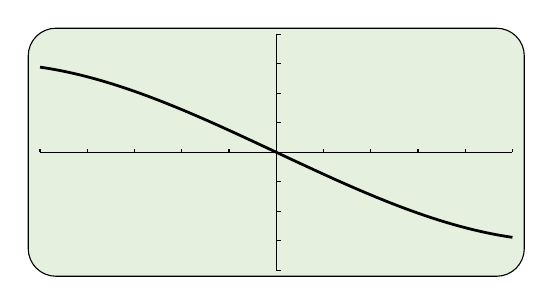
\begin{tikzpicture}[scale=0.5,x=1.2cm,y=0.75cm]
        \draw[rounded corners=10,fill = OliveGreen!10] (-5.25,-4.2) rectangle (5.25,4.2);
        \draw (-5,0) -- (5,0); \foreach \x in {-5,...,5} \draw (\x,0) -- (\x,0.1);
        \draw (0,-4) -- (0,4); \foreach \x in {-4,...,4} \draw (0,\x) -- (0.1,\x);
        \draw[smooth,samples=200,domain=-5:5, line width = 1pt] plot(\x,{(\x)^3/144 - 3*(\x)/4});
    \end{tikzpicture}
\end{center}

\begin{itemize}
    \item Sur quel intervalle est représentée la courbe de $f$ ?
    \item Quel est l'ensemble de définition de la fonction $f$ ?
    \item Paul affirme : << $f$ est décroissante sur $\R$ >>. A-t-il raison ? Justifier précisément.
\end{itemize}\[*\]

\exo

Voici la courbe obtenue à l'écran d'une calculatrice pour la fonction $g$ définie sur $\intervalleff{3}{3}$ par :
\[g(x) = \frac 1 4 x^4 + \frac13 x^3 - x^2.\]

\begin{center}
    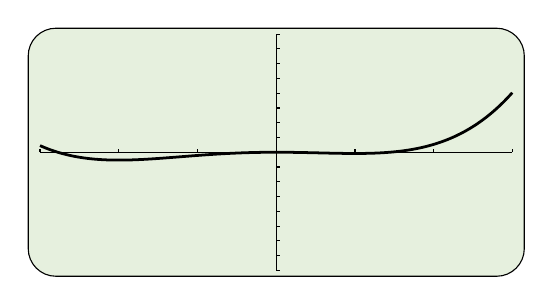
\begin{tikzpicture}[scale=0.5,x=2cm,y=0.75cm]
        \draw[rounded corners=10,fill = OliveGreen!10] (-3.15,-4.2) rectangle (3.15,4.2);
        \draw (-3,0) -- (3,0); \foreach \x in {-3,...,3} \draw (\x,0) -- (\x,0.1);
        \draw (0,-4) -- (0,4); \foreach \x in {-4,-3.5,...,4} \draw (0,\x) -- (0.05,\x);
        \draw[smooth,samples=200,domain=-3:3, line width = 1pt] plot(\x,{((\x)^4/4 + (\x)^3/3 - (\x)^2)/10});
    \end{tikzpicture}
\end{center}

La configuration de la fenêtre graphique n'est pas connue.

Paulette affirme : << $g$ est décroissante sur $\intervalleff{-3}{-2}$ puis croissante sur $\intervalleff{-2}{3}$.\par
A-t-elle raison ? Justifier précisément.

\end{document}
